\documentclass[11pt]{article}
\usepackage[a4paper,margin=0.9in]{geometry}
\usepackage{amsmath,amssymb,booktabs,graphicx,enumitem,xcolor,array,tikz}
\usepackage[hidelinks]{hyperref}
\usepackage{caption}
\setlength{\parindent}{0pt}\setlength{\parskip}{5pt}
\setlist{itemsep=2pt,topsep=3pt}
\renewcommand{\arraystretch}{1.2}
\newcommand{\T}{^{\top}}

\title{\textbf{Eigenfaces vs Fisherfaces: Project Report}}
\author{CS 740}
\date{}
\begin{document}
\maketitle
\vspace{-1.2em}

We reproduced Belhumeur, Hespanha and Kriegman, ``Eigenfaces vs.\ Fisherfaces'' (IEEE TPAMI 1997) in MATLAB, confirmed its main claim on Yale, found where it fails (ORL), and ran three experiments of our own. Every number below is printed by the three submitted scripts and appears in the \texttt{run\_log} files.

\section{Problem and algorithm}
The paper claims that Fisherfaces (PCA followed by LDA) recognise faces far more reliably than Eigenfaces (PCA) when lighting changes, because LDA uses the labels to discount variation within a person.
\begin{itemize}
\item \textbf{Eigenfaces:} subtract the mean face, keep the top $k$ eigenvectors of the total scatter $S_T$, project, classify by 1-nearest neighbour. PCA maximises $|W\T S_TW|$, so it keeps lighting variation too.
\item \textbf{Fisherfaces:} subtract the mean, reduce with PCA to $m$ dimensions (the paper uses $m=N-c$), solve $S_Bw=\lambda S_Ww$, keep the top $c-1$ directions, then 1-NN. LDA maximises $|W\T S_BW|/|W\T S_WW|$.
\item \textbf{Why PCA first:} $\operatorname{rank}S_W\le N-c$, far below the number of pixels $d$, so $S_W$ is singular in pixel space and $J$ is undefined.
\end{itemize}

\begin{center}
\begin{tabular}{lll}\toprule
 & ORL & Cropped Extended Yale B\\\midrule
Subjects used & 32 & 38\\
Images per subject & 10 (6 train / 4 test) & 59--64 (40 train)\\
Image size (pixels) & $92\times112=10{,}304$ & $168\times192=32{,}256$\\
What varies & pose, expression, glasses & lighting only\\\bottomrule
\end{tabular}
\end{center}
The two databases are near-complements, so together they act as a controlled experiment.

\textbf{What we implemented.} The Fisherfaces algorithm in full, plus three of the paper's four methods:
\begin{itemize}
\item \textbf{Correlation}, the paper's raw-pixel 1-nearest-neighbour baseline.
\item \textbf{Eigenfaces}, including the ``drop the first three components'' variant.
\item \textbf{Fisherfaces}.
\end{itemize}

\textbf{What we did not.} The Linear Subspace method of Section 2.3, which builds a separate 3-D illumination subspace per person.

\textbf{Different data.} The paper's lighting experiment uses the Harvard database, which has no surviving public download, and its Yale set is a smaller 1997 database. Cropped Extended Yale B is the successor of that set. The 38-subject extension is due to Lee, Ho and Kriegman (TPAMI 2005), Kriegman being an author of the 1997 paper, and the 10-subject Yale B before it to Georghiades, Belhumeur and Kriegman (TPAMI 2001). So our Yale comparison is \emph{modelled on} the paper's lighting experiment rather than a reproduction of it. Our glasses experiment uses ORL, where the paper used 36 paired Yale images, and that difference turns out to matter.

\section{The mathematics}
Each image is flattened column-by-column into $x_i\in\mathbb R^d$. There are $N$ training images in $c$ classes; class $j$ has $n_j$ images and mean $\mu_j$, and $\mu$ is the overall mean.

\textbf{Scatter matrices.} Total spread, spread between class means, and spread within each class:
\[
S_T=\sum_{i=1}^{N}(x_i-\mu)(x_i-\mu)\T,\qquad
S_B=\sum_{j=1}^{c}n_j(\mu_j-\mu)(\mu_j-\mu)\T,\qquad
S_W=\sum_{j=1}^{c}\sum_{x_i\in X_j}(x_i-\mu_j)(x_i-\mu_j)\T .
\]
Writing $x_i-\mu=(x_i-\mu_j)+(\mu_j-\mu)$ and noting the cross terms sum to zero within each class gives $S_T=S_B+S_W$.

\textbf{Eigenfaces (PCA)} keep the directions of largest total spread, i.e.\ the top eigenvectors of $S_T$. Forming $S_T$ explicitly is impossible for Yale ($32{,}256^2$ doubles, about $8.3$\,GB), so the code works through the $N\times N$ matrix $X\T X$ instead and maps the result back; the recovered columns have norm $\sqrt\lambda$ rather than $1$ and are renormalised, or the projection would stop being orthogonal.

\textbf{Fisherfaces (LDA)} maximise between-class spread relative to within-class spread:
\[ W_{fld}=\arg\max_W\;\frac{|W\T S_BW|}{|W\T S_WW|}. \]
For one direction the ratio is unchanged by scaling $w$, so fix the denominator and use a Lagrange multiplier:
\[ \max_w\; w\T S_Bw\ \ \text{s.t.}\ \ w\T S_Ww=1\;\Longrightarrow\; S_Bw=\lambda S_Ww,\qquad \lambda=\frac{w\T S_Bw}{w\T S_Ww}. \]
Each generalised eigenvalue \emph{is} the Fisher score of its direction, so we keep the largest. With two classes this has the closed form $w\propto S_W^{-1}(\mu_1-\mu_2)$, which is the two-class case the toy demonstration uses.

\textbf{Two rank bounds drive the whole method.} $\operatorname{rank}S_B\le c-1$, because $\sum_jn_j(\mu_j-\mu)=0$ makes the $c$ class-mean vectors linearly dependent, so there are \emph{at most $c-1$ Fisherfaces, whatever $d$ and $N$ are}. And $\operatorname{rank}S_W\le N-c$, because within class $j$ the deviations sum to zero and contribute only $n_j-1$ directions. Read the second as degrees of freedom: ORL gives 5 per person, Yale 39. Combining the two, $m$ is squeezed from both sides,
\[ c-1\;\le\;m\;\le\;N-c,\qquad W_{opt}=W_{pca}W_{fld},\quad W_{pca}\in\mathbb R^{d\times m},\ W_{fld}\in\mathbb R^{m\times(c-1)}, \]
the lower bound because $c-1$ directions cannot be pulled out of a space with fewer than $c-1$ dimensions. We found that one by crashing the Experiment 1 sweep at $m=20$.

\textbf{Solving $S_Bw=\lambda S_Ww$.} $S_W^{-1}S_B$ is not symmetric (its transpose is $S_BS_W^{-1}$), so the clean route factors $S_W=R\T R$ (Cholesky) and substitutes $w=R^{-1}z$, giving a symmetric ordinary eigenproblem with real eigenvalues and orthogonal eigenvectors:
\[ \left(R^{-\top}S_BR^{-1}\right)z=\lambda z,\qquad w=R^{-1}z,\qquad w_i\T S_Ww_j=0\ (i\ne j). \]
The paper specifies none of this. It says only ``the generalized eigenvectors of $S_B$ and $S_W$'', so the solver is our choice. The code calls \texttt{eig(Sb,Sw)}.


\textbf{Lighting, and the angle we measure.} A Lambertian patch with albedo $\rho$ and unit normal $n$, lit by a distant source $s$, has intensity $I=\rho\max(n\T s,0)$. Drop the $\max$ and stack all $d$ pixels: $x=Bs$, where $B$ depends only on the face and $s$ only on the lamp. One person's images under all lightings therefore lie in a subspace of dimension at most \textbf{3}, however many pixels there are. That is why illumination is \emph{structured} nuisance, the kind LDA can divide out, and it is the argument behind discarding the first three eigenfaces. The $\max$ we dropped is attached shadow, and cast shadows are not modelled at all, so past roughly $60^\circ$ off axis a large part of the face is dark and this linear picture no longer holds.

\textbf{The angle.} Yale gives the lamp as an \emph{azimuth} and an \emph{elevation}: azimuth is measured in the horizontal plane from the optical axis, elevation is the rise above that plane. With the camera looking along $z$,
\[ \frac{s}{\|s\|}=\bigl(\cos\mathrm{el}\sin\mathrm{az},\ \sin\mathrm{el},\ \cos\mathrm{el}\cos\mathrm{az}\bigr). \]
Write $\theta$ for the angle between $s$ and the optical axis. It is the inverse cosine of the $z$ component,
\[ \theta=\arccos\!\left(\cos\mathrm{el}\cdot\cos\mathrm{az}\right), \]
and it is $\theta$ that E3 bins on. For \texttt{yaleB01\_P00A+020E-40}, azimuth $+20^\circ$ and elevation $-40^\circ$ give $\theta=44.0^\circ$.
\begin{center}
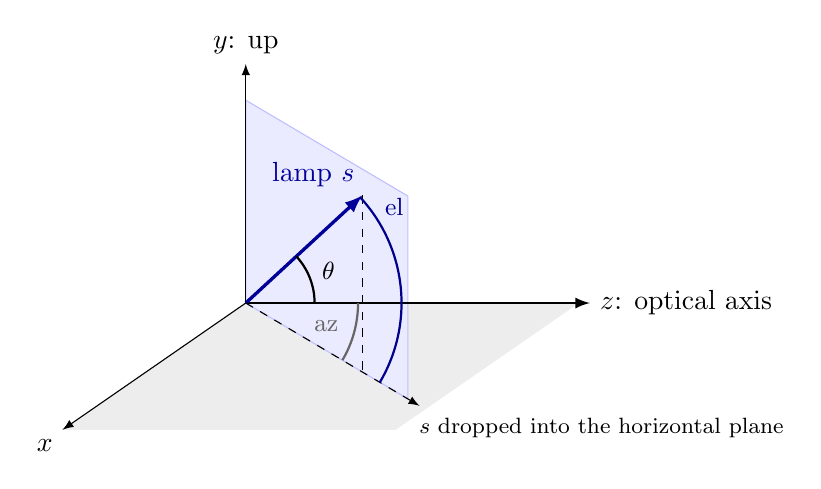
\begin{tikzpicture}[>=latex,scale=0.92]
% screen map: world (X,Y,Z) -> 4.6*(Z-0.55X, Y-0.38X).  Lamp drawn at az = 40, el = 32.
\fill[black!7] (0,0) -- (4.6,0) -- (2.07,-1.75) -- (-2.53,-1.75) -- cycle;
\fill[blue!8] (0,0) -- (2.237,-1.323) -- (2.237,1.477) -- (0,2.8) -- cycle;
\draw[blue!25] (0,0) -- (2.237,-1.323) -- (2.237,1.477) -- (0,2.8) -- cycle;
\draw[->,thick] (0,0) -- (4.75,0) node[right] {$z$: optical axis};
\draw[->] (0,0) -- (-2.53,-1.75) node[below left] {$x$};
\draw[->] (0,0) -- (0,3.3) node[above] {$y$: up};
\draw[->,very thick,blue!60!black] (0,0) -- (1.610,1.486) node[above left=-1pt] {lamp $s$};
\draw[dashed] (1.610,1.486) -- (1.610,-0.952);
\draw[->,dashed] (0,0) -- (2.40,-1.420);
\node[font=\footnotesize,anchor=north west] at (2.26,-1.45) {$s$ dropped into the horizontal plane};
\draw[thick] (0.95,0) arc (0:42.71:0.95);
\node[font=\small] at (1.14,0.44) {$\theta$};
\draw[thick,black!60] (1.55,0) arc (0:-30.59:1.55);
\node[font=\small,black!60] at (1.11,-0.32) {$\mathrm{az}$};
\draw[thick,blue!55!black] (1.851,-1.094) arc (-30.59:42.71:2.15);
\node[font=\small,blue!55!black] at (2.05,1.33) {$\mathrm{el}$};
\end{tikzpicture}
\captionof{figure}{Azimuth is measured in the horizontal plane, from the optical axis round to $s$ dropped into that plane. Elevation is the rise of $s$ above the plane. $\theta$ is the angle between $s$ and the optical axis, and it is what the subsets are binned on.}
\end{center}

\section{Implementation}
Three scripts, each with its helper functions at the bottom: \texttt{toy.m} (the 2-D demonstration), \texttt{eigenfaces\_vs\_fisherfaces.m} (the main comparison) and \texttt{experiments.m} (E1--E3). Base MATLAB only, no toolboxes.

\textbf{Eigenfaces.} Load and flatten with \texttt{im(:)}; centre on the mean face to get $X$; form $L=X\T X$; \texttt{eig} and sort \emph{descending} (MATLAB returns ascending); map the eigenvectors $V$ of $L$ back with $W_{pca}=XV$ and normalise each column; drop the last (eigenvalue 0, since $\operatorname{rank}X\le N-1$); project with the first $k$ columns of $W_{pca}$ and classify by 1-NN on squared distance, with test images centred on the \emph{training} mean.

\textbf{Fisherfaces.} Centre as above; PCA to $m$ dimensions giving $Z=W_{pca}\T X$, whose overall mean is zero because $X$ was centred; write $\bar z_j=W_{pca}\T(\mu_j-\mu)$ for the mean of class $j$ in that space and accumulate $S_B\mathrel{+}=n_j\bar z_j\bar z_j\T$ and $S_W\mathrel{+}=(z_i-\bar z_j)(z_i-\bar z_j)\T$ over classes, both $m\times m$ and never $d\times d$; solve $S_Bw=\lambda S_Ww$, sort descending, keep $c-1$ columns as $W_{fld}$; compose $W_{opt}=W_{pca}W_{fld}$; unit-normalise its columns; project and classify.

\begin{center}
\begin{tabular}{@{}lll@{}}\toprule
Matrix & Size & ORL ($N=192$, $c=32$)\\\midrule
$X$ (centred images) & $d\times N$ & $10{,}304\times192$\\
$L=X\T X$ & $N\times N$ & $192\times192$\\
$W_{pca}$ & $d\times m$ & $10{,}304\times160$\\
$S_B,\ S_W$ (reduced) & $m\times m$ & $160\times160$\\
$W_{opt}$ (Fisherfaces) & $d\times(c-1)$ & $10{,}304\times31$\\\bottomrule
\end{tabular}
\end{center}

\section{Main result}
Fisherfaces roughly double Eigenfaces on Yale and lose on ORL.
\begin{center}\small
\begin{tabular}{@{}lccccc@{}}\toprule
Recognition rate (\%) & Correlation & Eigen (best $k$) & Eigen ($k{=}c{-}1$) & Eigen w/o top 3 & Fisherfaces\\\midrule
Yale-38 & 42.95 & 34.23 & 29.53 & 58.72 & \textbf{67.23}\\
ORL-32 & 91.41 & \textbf{95.31} & 94.53 & 87.50 & 90.62\\\bottomrule
\end{tabular}
\end{center}
Fisherfaces always use exactly $c-1$ features, so the $k=c-1$ column is the fair comparison. Dropping the top three eigenfaces raises Yale from 34.23 to 58.72, because those components encode lighting, and \emph{hurts} ORL (95.31 to 87.50), where they encode identity. That sign flip is the paper's argument in miniature, and Fisherfaces still beat the drop-3 trick on Yale, because that trick assumes the nuisance is exactly 3-dimensional while LDA learns it from the labels.

\textbf{Why Fisherfaces lose on ORL}, and they lose to raw-pixel correlation too. Eigenfaces never estimates $S_W$: it keeps the \emph{largest} eigenvalues of a well-estimated $S_T$. Fisherfaces must \emph{invert} $S_W$, so it leans on the \emph{smallest} eigenvalues, which are the worst estimated. ORL supplies only 5 degrees of freedom per person against Yale's 39.

\begin{center}
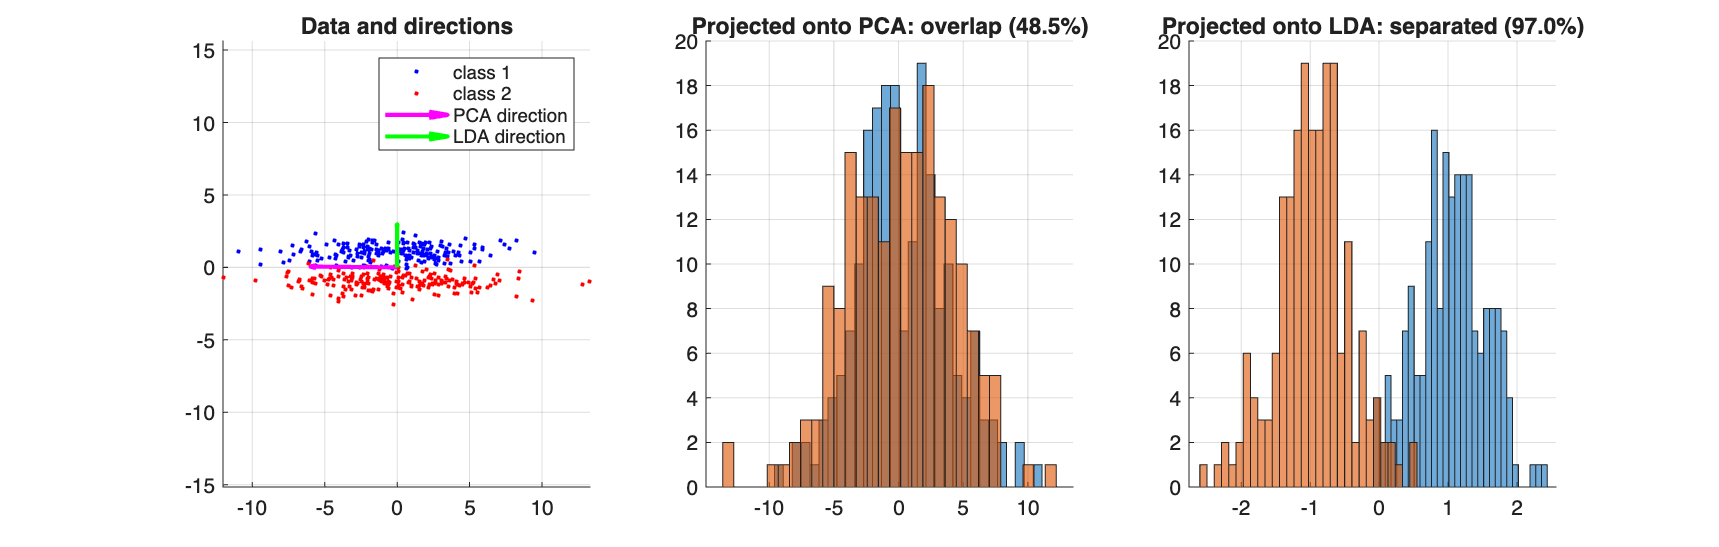
\includegraphics[width=0.95\textwidth]{figures/toy.png}\\[4pt]
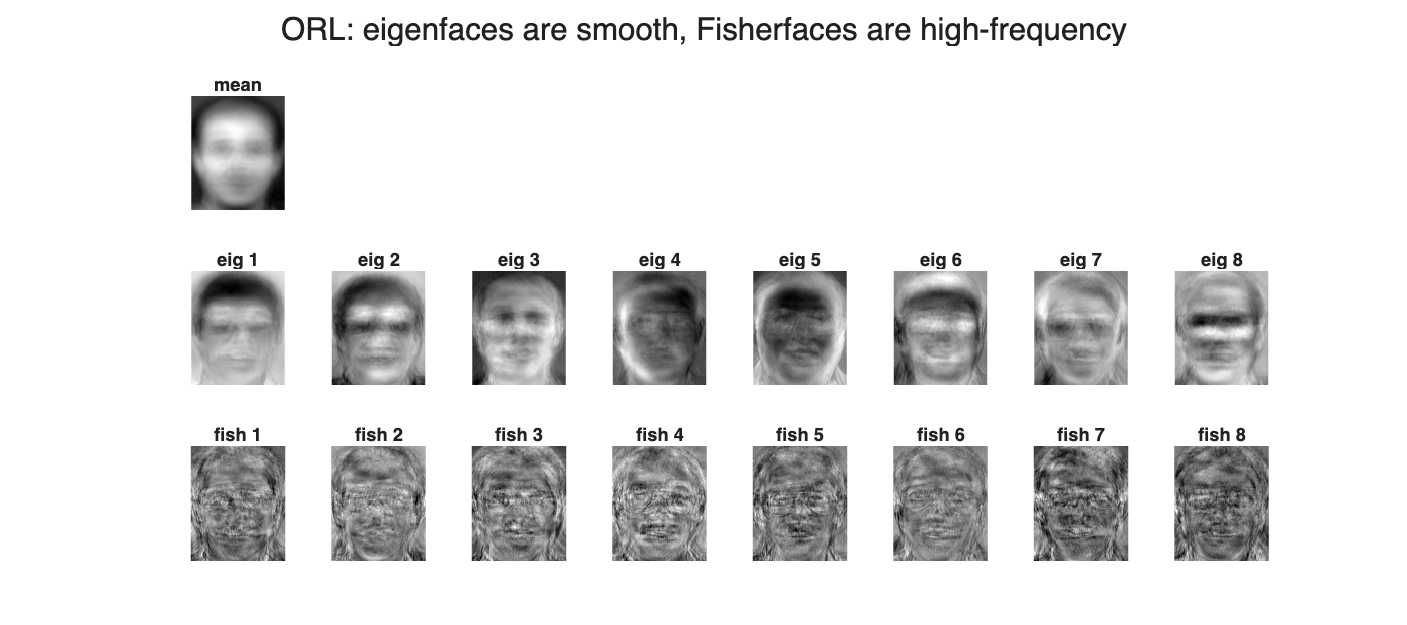
\includegraphics[width=0.88\textwidth]{figures/ORL_faces.png}
\captionof{figure}{Top: the 2-D toy problem. All the spread is along $x$ and all the class information along $y$, so PCA picks the useless direction (48.5\% error, chance 50\%) and Fisher the useful one (97.0\%). Bottom: ORL mean face, first eight eigenfaces and first eight Fisherfaces.}
\end{center}

\begin{center}
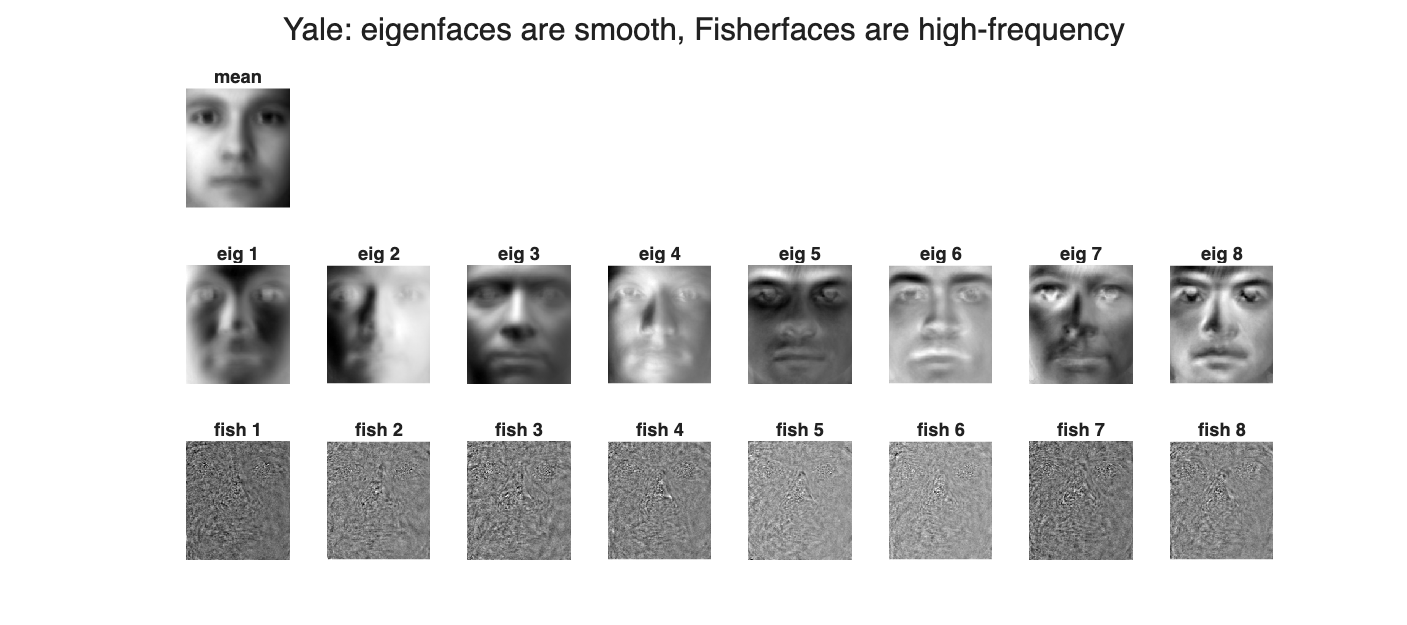
\includegraphics[width=0.97\textwidth]{figures/Yale_faces.png}
\captionof{figure}{Yale: eigenfaces are smooth and face-like, Fisherfaces are speckled and concentrate around the eyes and brow. This is predicted, not incidental: whitening scales each eigen-direction of $S_W$ by $1/\sqrt\lambda$, and the small-$\lambda$ directions are the high-frequency ones.}
\end{center}

\section{Experiments}

\subsection{E1: Choosing the PCA dimension $m$}
The paper fixes $m=N-c$, where $S_W$ has rank $m$ exactly: full rank with \emph{zero slack}, one direction away from singular. Sweeping $m$ and recording $\kappa(S_W)$, the ratio of largest to smallest eigenvalue:
\begin{center}\small
\begin{tabular}{rrr@{\hskip 2.2em}rrr}\toprule
\multicolumn{3}{c}{\textbf{ORL} ($N-c=160$)} & \multicolumn{3}{c}{\textbf{Yale} ($N-c=1482$)}\\
$m$ & rate (\%) & $\kappa(S_W)$ & $m$ & rate (\%) & $\kappa(S_W)$\\\midrule
31 & 94.5 & $6.5\times10^{1}$ & 100 & 51.6 & $3.6\times10^{3}$\\
60 & \textbf{95.3} & $1.8\times10^{2}$ & 400 & 65.2 & $4.9\times10^{4}$\\
120 & 90.6 & $1.7\times10^{3}$ & 1000 & \textbf{69.8} & $1.1\times10^{6}$\\
140 & 89.1 & $5.8\times10^{3}$ & 1200 & 69.4 & $3.6\times10^{6}$\\
160 & 90.6 & $\mathbf{7.9\times10^{7}}$ & 1482 & 67.2 & $\mathbf{6.0\times10^{12}}$\\\bottomrule
\end{tabular}
\end{center}
\textbf{The paper's $m=N-c$ is not the best choice on either database.} ORL peaks at $m=60$ (95.3 vs 90.6), Yale at $m=1000$ (69.8 vs 67.2). Accuracy turns down well before conditioning becomes alarming, so the extra directions are fitting noise, not only losing precision. Note what this table is: the best $m$ is being read off the test column, which is tuning on test, so 95.3\% is an optimistic figure rather than an honest estimate of accuracy on unseen faces.

\begin{center}
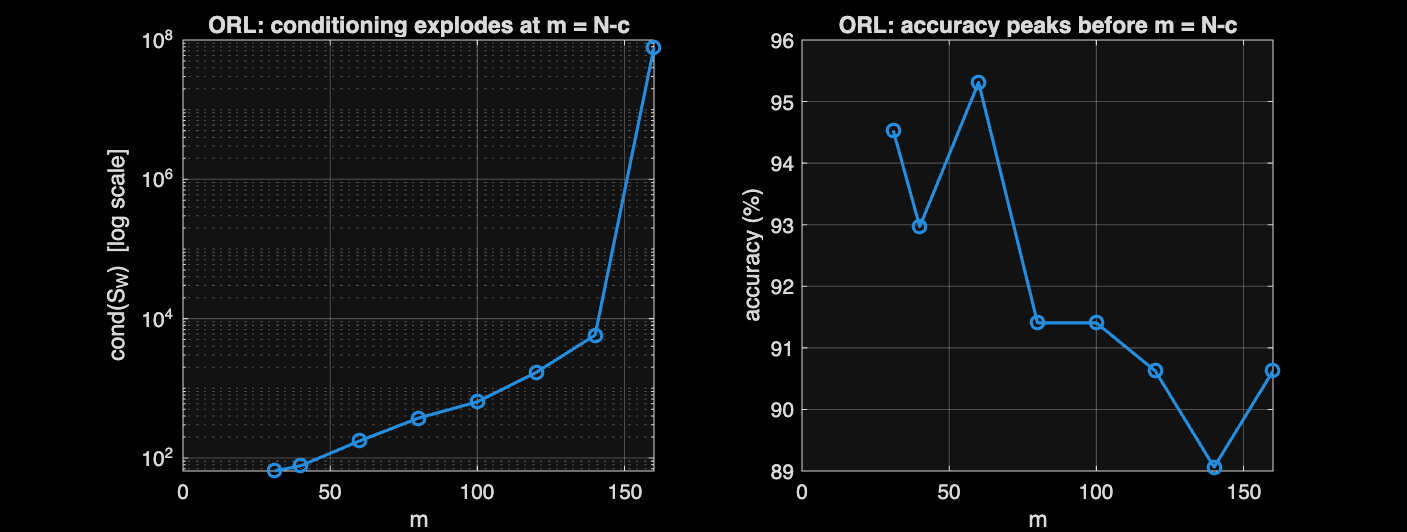
\includegraphics[width=0.92\textwidth]{figures/E1_sweep_m_ORL.png}\\[2pt]
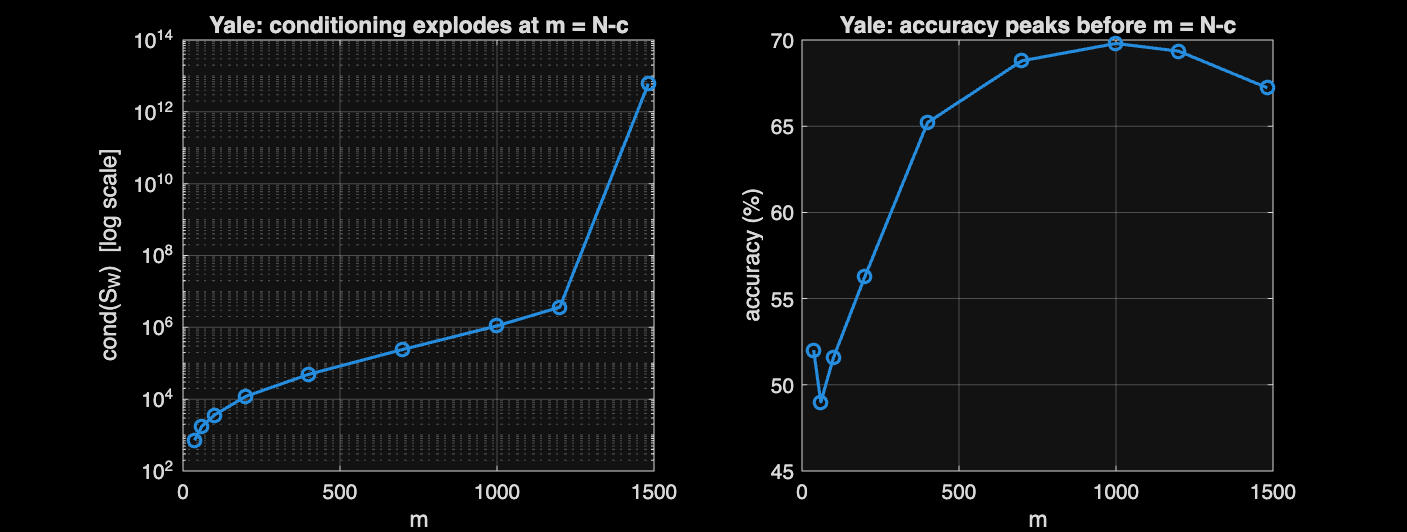
\includegraphics[width=0.92\textwidth]{figures/E1_sweep_m_Yale.png}
\captionof{figure}{Condition number of $S_W$ (left, log scale) and recognition rate (right) against $m$, for ORL (top) and Yale (bottom).}
\end{center}

\subsection{E2: Glasses or no glasses}
A different question, and the paper's Section 3.3: not \emph{who} is this, but \emph{is this person wearing glasses}. With $c=2$, $\operatorname{rank}S_B\le1$ and there is exactly \textbf{one} Fisherface, $w\propto S_W^{-1}(\mu_1-\mu_2)$, so the whole decision rests on a single direction.

\textbf{Both methods share one pipeline.} We first project, with PCA or with LDA, and then classify by 1-nearest neighbour, using the glasses label in place of the identity label. Only the projection differs. PCA picks its directions by total variance and never sees a label, so it can succeed only if glasses account for a large share of that variance. They do not: a pair of frames is a small, localised, high-frequency detail, and the leading $k=10$ components are exactly where such detail is discarded. LDA picks the single direction that best separates the two labelled groups while discounting the variation inside them. The comparison therefore isolates one thing, whether using the labels to choose the directions helps.

ORL ships no glasses labels, so we labelled all 400 images by inspection: 117 wear glasses and 8 people appear both with and without, which is what makes the question non-trivial. On the raw set, always answering ``no'' scores 70.8\% and beats any real method, so we balanced it to 234 images (50/50) and used leave-one-\emph{subject}-out: the test face is never seen in training, so the classifier cannot cheat by recognising the person.

\textbf{One balanced subset is not an experiment.} Which 117 no-glasses images get drawn moved the Fisherface error from 35.9\% to 50.9\%, so we average over ten draws and report the range too.
\begin{center}
\begin{tabular}{lccc}\toprule
Error (\%) & Ours (mean of 10) & Range & Paper (Yale, 36 images)\\\midrule
PCA ($k=10$) & 43.1 & 37.2--48.3 & 52.6\\
One Fisherface & \textbf{41.5} & 35.9--50.9 & \textbf{5.3}\\
Always answer ``no'' & 50.0 & n/a & 50.0\\\bottomrule
\end{tabular}
\end{center}
\textbf{We reproduce the paper's finding that PCA is near chance, but not that Fisherfaces solve the task.} We think the difference is the data, not the method: the paper's 36 images were \emph{paired}, the same person photographed with and without glasses in one session under the same lighting, so glasses were the only thing that changed. In ORL glasses co-vary with pose, expression and session, so the single Fisher direction has no clean signal to lock onto. This is a negative result and we report it as one.
\begin{center}
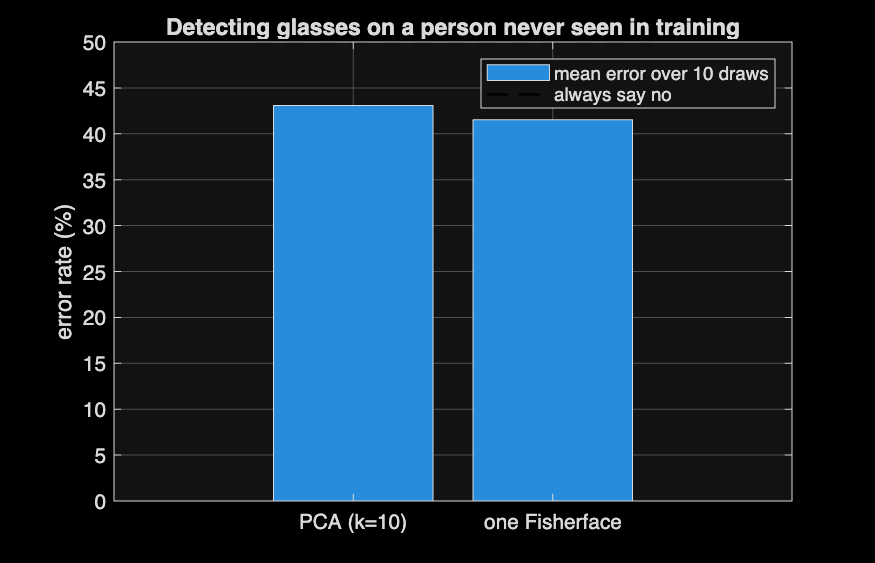
\includegraphics[width=0.48\textwidth]{figures/E2_glasses.png}
\captionof{figure}{Mean error over ten balanced draws on a person never seen in training; the dashed line is the 50\% a coin achieves.}
\end{center}

\subsection{E3: Error against lighting angle}
The paper does not report one Yale number; it bins the test images by $\theta$, the angle of the lamp off the optical axis defined in Section 2. The five bins are the standard subsets of the Yale B literature.
\begin{center}
\begin{tabular}{lccccc}\toprule
Error (\%) & $0$--$12^\circ$ & $13$--$25^\circ$ & $26$--$50^\circ$ & $51$--$77^\circ$ & $>77^\circ$\\
Test images & 0 & 104 & 152 & 300 & 338\\\midrule
Eigenfaces & n/a & 1.0 & 30.9 & 88.3 & 93.8\\
Fisherfaces & n/a & \textbf{0.0} & \textbf{2.0} & \textbf{22.0} & \textbf{66.3}\\\bottomrule
\end{tabular}
\end{center}
Error climbs with angle for both methods and the gap \emph{widens}: at $26$--$50^\circ$ Fisherfaces are $15\times$ better, and even in the hardest bin they halve the error. This is the paper's central claim measured where it bites rather than averaged into one number.

\textbf{Why the first bin is empty.} This is a property of the split, not of the parser, and the chain is worth following. A subject with the full 64 images has 35 taken with positive azimuth and 29 with negative. The loader keeps the first 40 files that \texttt{dir} returns, and \texttt{dir} sorts names as text rather than by angle, with the character \texttt{'+'} ordering before \texttt{'-'}. Every \texttt{A+} file therefore sorts ahead of every \texttt{A-} file, so the first 40 are all 35 positive-azimuth images together with the 5 negative ones nearest zero (down to \texttt{A-015}). Those 40 contain every near-frontal lamp in the database. Testing is left with the far side only, starting at \texttt{A-020}: no test image falls within $12^\circ$ of the axis, which is why the first bin is empty, and 638 of the 894 lie beyond $50^\circ$. The Yale rates in this report are therefore measured on the hard tail of the lighting distribution rather than on a representative sample of it.

\begin{center}
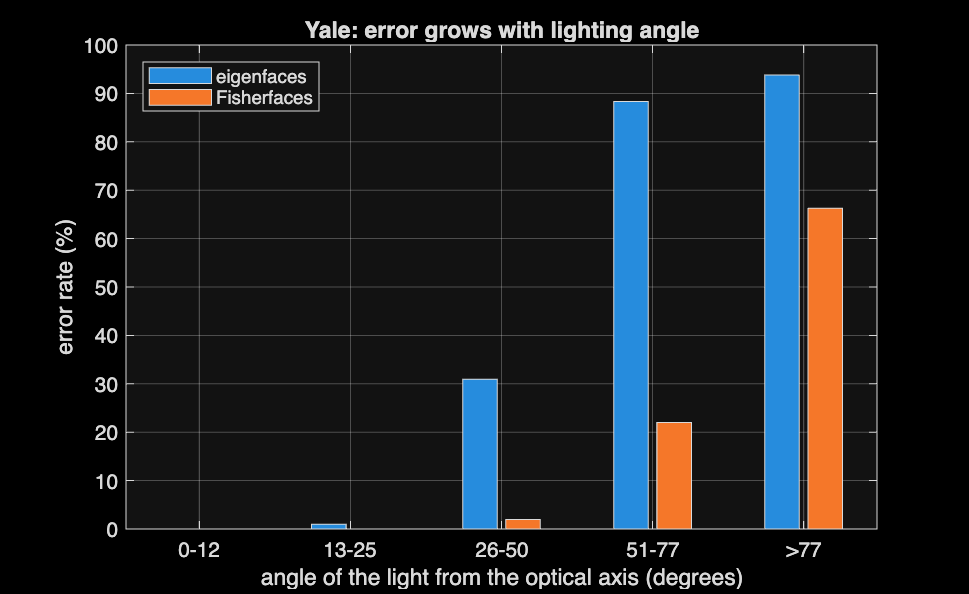
\includegraphics[width=0.56\textwidth]{figures/E3_lighting_angle.png}
\captionof{figure}{Error against lighting angle. The first bin is a gap, not a zero bar, because it holds no test images.}
\end{center}

\section{Conclusions}
\begin{enumerate}
\item \textbf{The paper's claim holds where the within-person nuisance is large and structured.} Under lighting change Fisherfaces take Yale from 34.23\% to 67.23\%, nearly doubling the recognition rate, and are $15\times$ better than Eigenfaces in the $26$--$50^\circ$ bin.
\item \textbf{It is a claim about nuisance structure, not ``LDA is always better''.} On ORL, which varies by pose and expression with 6 images per person, Eigenfaces win, and Fisherfaces lose even to raw-pixel correlation. What decides the outcome is how much \emph{structured} within-class variation there is for LDA to discount, not the algorithm.
\item \textbf{$m=N-c$ is the weakest part of the recipe.} It is the worst-conditioned valid choice, and a smaller $m$ does better on both databases. The blow-up at $\gamma\to1$ is predicted by Marchenko--Pastur, so this is not a quirk of our data.
\end{enumerate}

\end{document}
